
\documentclass[11pt]{article}
\usepackage[margin=1in]{geometry}

% Core packages
\usepackage{amsmath,amssymb}
\usepackage{tikz-cd}
\usetikzlibrary{positioning,arrows.meta}
\usepackage{multicol}
\usepackage[T1]{fontenc}
\usepackage[utf8]{inputenc}
\usepackage{lmodern}
\usepackage{microtype}
\usepackage{enumitem}
\usepackage{hyperref}
\usepackage{array}
\usepackage{ragged2e}
\usepackage{booktabs}
\usepackage{tabularx}
\usepackage[table]{xcolor}
\usepackage{titlesec}
\usepackage{fancyhdr}
\usepackage{float}
\usepackage[most]{tcolorbox}

% Paragraphs
\setlength{\parindent}{0pt}
\setlength{\parskip}{0.8\baselineskip}

% Styling
\definecolor{dverseblue}{HTML}{1F4E79}
\definecolor{dverselight}{HTML}{EAF2F8}
\definecolor{dverseborder}{HTML}{B8C9D9}
\hypersetup{
    colorlinks=true,
    linkcolor=dverseblue,
    urlcolor=dverseblue,
    citecolor=dverseblue,
    pdftitle={DVerse Communication Platform: Research Design for a Distributed Human--AI Collaboration System},
    pdfauthor={Abel-Raul Mazilu}
}

\titleformat{\section}
  {\Large\bfseries\color{dverseblue}}
  {\thesection}{0.75em}{}
\titleformat{\subsection}
  {\large\bfseries\color{dverseblue}}
  {\thesubsection}{0.75em}{}
\titleformat{\subsubsection}
  {\normalsize\bfseries\color{dverseblue}}
  {\thesubsubsection}{0.75em}{}

\titlespacing*{\section}{0pt}{1.2\baselineskip}{0.5\baselineskip}
\titlespacing*{\subsection}{0pt}{1\baselineskip}{0.35\baselineskip}
\titlespacing*{\subsubsection}{0pt}{0.8\baselineskip}{0.25\baselineskip}

\setlist[itemize]{leftmargin=1.5em,itemsep=0.3em,topsep=0.4em}
\setlist[enumerate]{leftmargin=1.8em,itemsep=0.5em,topsep=0.5em}

\pagestyle{fancy}
\fancyhf{}
\fancyhead[L]{\textit{DVerse Communication Platform}}
\fancyhead[R]{\thepage}
\renewcommand{\headrulewidth}{0.4pt}
\setlength{\headheight}{14pt}

\newtcolorbox{abstractbox}{
    colback=dverselight,
    colframe=dverseblue!65,
    boxrule=0.8pt,
    arc=3pt,
    left=10pt,
    right=10pt,
    top=10pt,
    bottom=10pt
}

\title{DVerse Communication Platform: \\
Research Design for a Distributed Human--AI Collaboration System}
\author{Abel-Raul Mazilu}
\date{\today}

\begin{document}
\maketitle

\thispagestyle{empty}

\begin{center}
    {\large\color{dverseblue}\textbf{Research Design Document}}
\end{center}

\begin{abstractbox}
\begin{abstract}
\large
This research design document is intended to report findings throughout the course of the research project and to provide a clear direction for the continued development of the DVerse communication platform. It outlines the project's objectives, research questions, architectural choices, and evaluation approach so that both the research process and the development process can move forward in a structured and coherent way.
\end{abstract}
\end{abstractbox}

\section*{Version History}

\begin{center}
\renewcommand{\arraystretch}{1.2}
\rowcolors{2}{dverselight}{white}
\begin{tabularx}{0.9\textwidth}{>{\raggedright\arraybackslash}p{0.15\textwidth}>{\raggedright\arraybackslash}p{0.2\textwidth}X}
    \rowcolor{dverseblue!15}
    \toprule
    \textbf{Version} & \textbf{Date} & \textbf{Changes} \\
    \midrule
    0.1 & 16 April 2026 & Initial draft of the research design document. \\
    0.2 & 4 May 2026 & Remade Research Document from Markdown into LaTeX, added Version History and Table of Contents, improved styling, answered SQ1, SQ2 and SQ3. \\
    0.3 & 1 June 2026 & Finished answering Research Questions. \\
    \bottomrule
\end{tabularx}
\end{center}
\newpage
\tableofcontents
\thispagestyle{empty}
\clearpage

\section{Introduction}

DVerse is a social communication platform intended to support collaboration between human participants and artificial agents. The platform is designed for small-group communication in which participants exchange information, co-create content, and make decisions in real time while receiving assistance from AI-driven components. The project is situated within the Interaction Design (IXD) research group of the Digital Communities programme, where the broader focus lies on human-centred design through digital technologies and artificial intelligence.

Earlier iterations of DVerse adopted a multi-chatroom model built on an event-driven architecture. While this approach enabled rapid experimentation, it also exposed architectural limitations related to scalability, flexibility, and the integration of increasingly sophisticated AI-supported interactions. In response, this research investigates a new architectural direction based on distributed publish--subscribe communication. The central premise is that a distributed pub-sub architecture may provide stronger foundations for real-time collaboration, modularity, and system evolution in hybrid human--AI environments.

This document presents the research objective, research questions, architectural approach, methodology, expected contributions, project scope, and alignment with learning outcomes. It reframes the project as both an engineering effort and a research inquiry into how modern distributed systems can meaningfully support collaborative digital environments.

\section{Research Objective}

The objective of this research is to design, implement, and evaluate a distributed communication platform architecture that enables scalable, secure, observable, and maintainable real-time collaboration between humans and AI agents. In addition, the study aims to validate the practical applicability of this architecture through the integration of an interactive collaboration game within the platform.

More specifically, the project seeks to determine whether a distributed pub-sub model can improve upon the limitations of the previous event-driven system while preserving usability and supporting richer forms of interaction between human users and artificial agents.

\section{Research Questions}

\subsection{Main Research Question}

How can a distributed, publish--subscribe-based architecture be designed and evaluated to support scalable, secure, observable, and maintainable real-time collaboration between humans and AI agents?

\subsection{Subquestions}

\begin{enumerate}[label=\textbf{SQ\arabic*}.]
    \item \textbf{Scalability and Performance.} How does the proposed architecture perform under increasing load in terms of latency, throughput, and system reliability compared to the existing event-driven system?
    \item \textbf{Observability.} How can observability be implemented in a distributed pub-sub system to effectively monitor system behaviour, detect failures, and support debugging in real-time collaboration scenarios?
    \item \textbf{Security.} What security mechanisms are required to ensure safe communication, authentication, and data integrity within a distributed multi-agent communication platform?
    \item \textbf{Maintainability.} How do architectural choices such as modular design, pub-sub communication, and system structure affect the maintainability and extensibility of the platform?
    \item \textbf{Human--AI Collaboration.} How do AI agents influence collaboration efficiency, decision-making quality, and user experience in small-group communication sessions?
    \item \textbf{Integration of the Collaboration Game.} What architectural and interaction design considerations are required to successfully integrate the DVerse Collaboration Game into the communication platform?
\end{enumerate}

Together, these questions connect technical system qualities with experiential and design-oriented concerns, ensuring that the research does not evaluate the architecture solely on implementation efficiency, but also on its suitability for collaborative human use.

\subsection{Answer to SQ1: Scalability and Performance}

An answer to \textbf{SQ1} is that a distributed publish--subscribe architecture is likely to provide stronger scalability and performance characteristics than the previous event-driven implementation, provided that it is designed and implemented with care. From an architectural perspective, publish--subscribe communication supports a greater degree of decoupling between producers and consumers, which in turn allows system components to be scaled more independently and reduces the risk of central bottlenecks \cite{eugster2003}.

In particular, the proposed use of a distributed communication mesh such as Zenoh suggests improved \textbf{horizontal scalability}. Because services communicate through published topics rather than direct point-to-point dependencies, additional consumers or service instances can be introduced as workload increases without requiring substantial restructuring of the system. This architectural flexibility is expected to support better load distribution across the platform.

A second expected improvement concerns \textbf{throughput and responsiveness}. In a pub-sub model, producers do not need to wait for consumers in the same way as in more tightly coupled architectures. This reduces blocking behaviour and may allow messages to be processed more efficiently under concurrent load. In combination with Rust's strong concurrency model, asynchronous execution support, and memory-safety guarantees, the new system is expected to achieve lower latency and more stable performance under stress than the previous Python-based implementation \cite{eugster2003}.

To evaluate this expectation, the research will focus on three principal performance dimensions:

\begin{itemize}
    \item \textbf{Latency} -- the time between message publication and message reception, which should remain relatively stable under moderate load and degrade gradually rather than abruptly under stress.
    \item \textbf{Throughput} -- the number of messages processed per second, which should increase as additional nodes or service instances are introduced, ideally approaching linear scaling within practical limits.
    \item \textbf{Reliability} -- the system's ability to minimise message loss and recover from partial failures while maintaining acceptable service continuity.
\end{itemize}

The anticipated contrast between the previous and proposed architectures is summarised in Table~\ref{tab:sq1-comparison}.

\begin{table}[H]
    \centering
    \renewcommand{\arraystretch}{1.2}
    \rowcolors{2}{dverselight}{white}
    \begin{tabularx}{0.95\textwidth}{>{\raggedright\arraybackslash}p{0.24\textwidth}>{\raggedright\arraybackslash}X>{\raggedright\arraybackslash}X}
        \rowcolor{dverseblue!15}
        \toprule
        \textbf{Aspect} & \textbf{Previous Event-Driven System} & \textbf{Proposed Distributed Pub-Sub System} \\\\        \midrule
        Coupling & Medium to high, with stronger interdependence between components & Low, with clearer separation between producers and consumers \\\\        Scalability & Limited by central bottlenecks and tighter service dependencies & Higher potential for horizontal scaling across distributed components \\\\        Latency under load & More likely to degrade rapidly as contention increases & Expected to remain more stable and degrade more gradually under stress \\\\        Fault isolation & Relatively weak, as failures may propagate more easily across the system & Stronger, because distributed components can fail more independently \\\\        \bottomrule
    \end{tabularx}
    \caption{Preliminary comparison between the previous event-driven architecture and the proposed distributed publish--subscribe architecture for SQ1.}
    \label{tab:sq1-comparison}
\end{table}

At the same time, this architectural advantage should not be interpreted as unconditional. The proposed system is also expected to introduce additional complexity, particularly in relation to message ordering, network overhead, and debugging in distributed execution contexts. For this reason, the research does not assume that the new architecture is automatically superior in every respect; rather, it hypothesises that the gains in scalability, fault isolation, and performance under load will outweigh the additional operational complexity when evaluated in realistic collaboration scenarios.

\subsection{Answer to SQ2: Observability}

An answer to \textbf{SQ2} is that observability must be treated as a first-class architectural concern in DVerse rather than as an auxiliary development feature. In a distributed publish--subscribe system, there is no single execution point from which the full system state can be inspected. Message flows are asynchronous, components are decoupled, and interactions may traverse multiple services, machines, and AI agents. As a result, effective monitoring and debugging depend on combining multiple observability techniques that together provide visibility into both system behaviour and development-time maintenance concerns.

The proposed observability approach is therefore based on three complementary mechanisms: \textbf{distributed tracing}, \textbf{structured logging}, and \textbf{metrics collection}. In practical terms, these are implemented primarily through OpenTelemetry and Pydantic Logfire. OpenTelemetry is particularly suitable for end-to-end tracing and metrics export across distributed services, whereas Pydantic Logfire is especially useful for structured, schema-aware logging in Python-based agent and AI components. Rather than competing tools, they are best understood as complementary layers within the same observability strategy \cite{opentelemetryDocs,logfireConcepts}.

The most important mechanism for understanding system behaviour is \textbf{distributed tracing with OpenTelemetry}. Each message or interaction can be associated with a trace identifier, and every component that handles the message contributes one or more spans to that trace. In DVerse, this would make it possible to reconstruct an end-to-end path such as router to agent to AI service and back to a user-facing component. This is especially valuable in publish--subscribe systems because interactions do not naturally form a simple request--response chain. Instead, traces allow the system to reconstruct asynchronous flows, identify latency bottlenecks, and locate the origin of failures. For example, if an AI response appears delayed, a trace can show whether the delay was caused by message routing, agent processing, or model inference time \cite{opentelemetryDocs,opentelemetrySpec}.

Tracing alone, however, does not fully explain what happened within each component. For that reason, \textbf{structured logging with Pydantic Logfire} forms a second major mechanism. Logfire is useful because it supports schema-validated logs that are consistent across components and easier to query than unstructured text logs. In the context of DVerse, structured log entries should include timestamps, service or agent identity, message or topic identifiers, and where possible the trace and span identifiers generated through OpenTelemetry. This creates a strong link between event-level detail and system-wide flow visibility. It is particularly helpful for debugging malformed messages, unexpected agent behaviour, and AI input-output handling, where developers need more contextual detail than a trace alone can provide \cite{logfireDocs,logfireConcepts}.

A third necessary dimension is \textbf{metrics collection}. While traces and logs are well suited to explaining individual behaviours, metrics provide a broader operational picture of system health over time. Relevant measures for DVerse include message latency percentiles such as p95 and p99, throughput in messages per second, error rates, and the number of active routers or agents. Exported through OpenTelemetry and visualised in dashboards, such metrics support real-time monitoring, alerting on abnormal behaviour, and performance comparisons under varying load conditions \cite{opentelemetryDocs,logfireConcepts}.

A central technical challenge in pub-sub systems is \textbf{context propagation across asynchronous boundaries}. In order for telemetry to remain meaningful, observability metadata such as trace identifiers, span identifiers, and timestamps must travel with messages as they move through the system. This allows each downstream component to continue an existing trace rather than creating disconnected telemetry fragments. Without such propagation, observability becomes partial and fragmented, making it difficult to analyse complete interaction chains.

When these mechanisms are combined, observability becomes a powerful tool not only for runtime monitoring but also for \textbf{software maintenance}. Tracing helps identify where a failure occurred, structured logging helps explain why it occurred, and metrics help determine how frequently it occurs and what broader effect it has on the system. This layered visibility improves debugging, shortens diagnosis time, and supports maintainability by making distributed behaviour more understandable for current and future developers. In that sense, observability contributes directly to maintainability: a system that can be inspected, queried, and analysed systematically is easier to extend, test, and repair.

The telemetry flow anticipated in the platform is illustrated in Figure~\ref{fig:sq2-telemetry-flow}.

\begin{figure}[H]
    \centering
    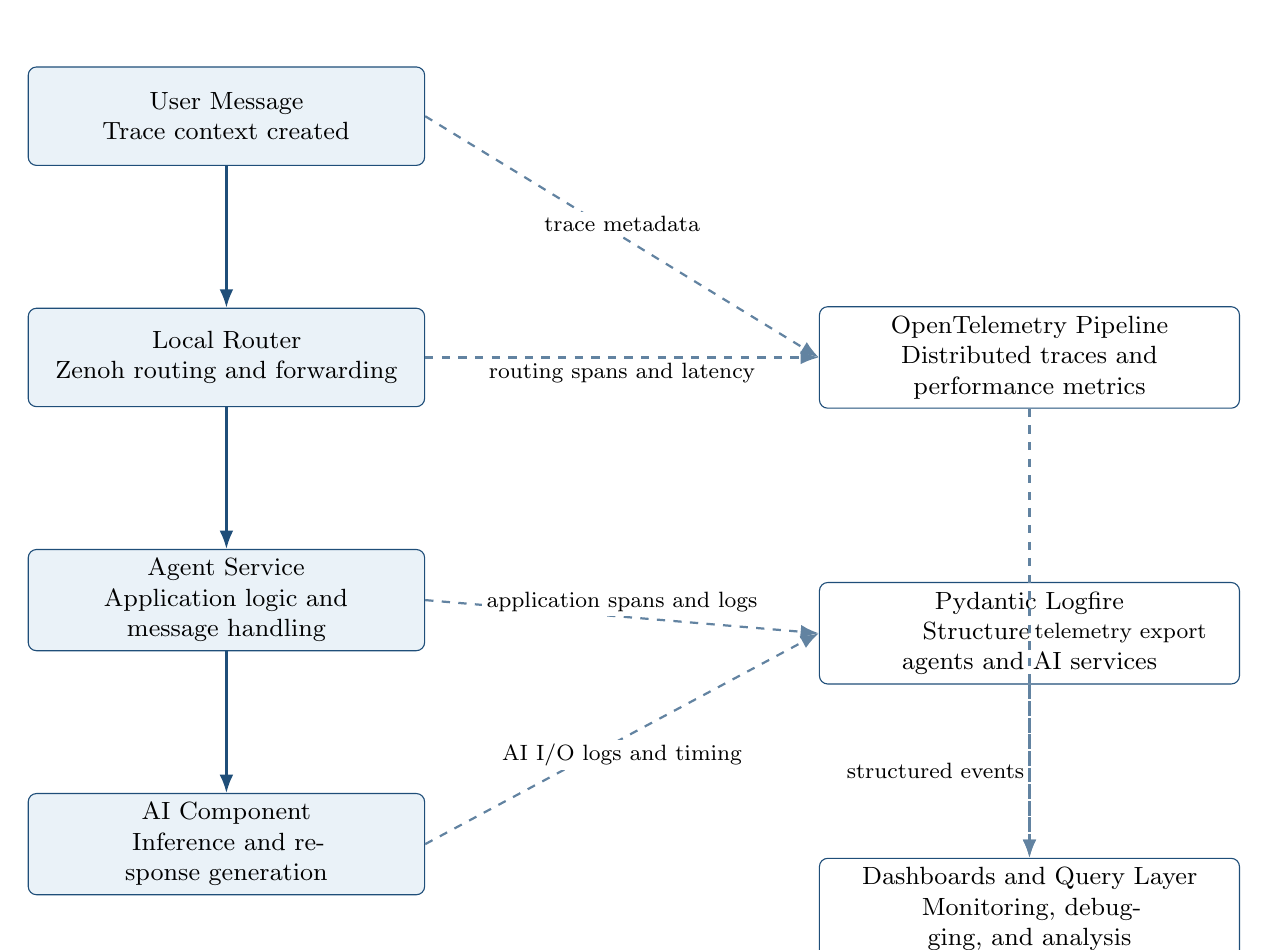
\begin{tikzpicture}[
        node distance=1.8cm and 5.0cm,
        >=Latex,
        every node/.style={font=\small},
        component/.style={draw=dverseblue, rounded corners=3pt, fill=dverselight, text width=4.8cm, minimum height=1.25cm, align=center},
        collector/.style={draw=dverseblue, rounded corners=3pt, fill=white, text width=5.1cm, minimum height=1.25cm, align=center},
        flow/.style={->, thick, color=dverseblue},
        telemetry/.style={draw=dverseblue!70, dashed, ->, thick},
        labeltext/.style={font=\footnotesize, fill=white, inner sep=1.5pt, align=center}
    ]
        \node[component] (user) {User Message\\Trace context created};
        \node[component, below=of user] (router) {Local Router\\Zenoh routing and forwarding};
        \node[component, below=of router] (agent) {Agent Service\\Application logic and message handling};
        \node[component, below=of agent] (ai) {AI Component\\Inference and response generation};

        \node[collector, right=of router] (otel) {OpenTelemetry Pipeline\\Distributed traces and performance metrics};
        \node[collector, below=2.2cm of otel] (logfire) {Pydantic Logfire\\Structured logs for agents and AI services};
        \node[collector, below=2.2cm of logfire] (dashboard) {Dashboards and Query Layer\\Monitoring, debugging, and analysis};

        \draw[flow] (user) -- (router);
        \draw[flow] (router) -- (agent);
        \draw[flow] (agent) -- (ai);

        \draw[telemetry] (user.east) -- (otel.west) node[midway, above, labeltext]{trace metadata};
        \draw[telemetry] (router.east) -- (otel.west) node[midway, below, labeltext]{routing spans and latency};
        \draw[telemetry] (agent.east) -- (logfire.west) node[midway, above, labeltext]{application spans and logs};
        \draw[telemetry] (ai.east) -- (logfire.west) node[midway, below, labeltext]{AI I/O logs and timing};
        \draw[telemetry] (otel) -- (dashboard) node[midway, right, labeltext]{telemetry export};
        \draw[telemetry] (logfire) -- (dashboard) node[midway, left, labeltext]{structured events};
    \end{tikzpicture}
    \caption{Illustrative telemetry flow for observability in DVerse when a message traverses the platform.}
    \label{fig:sq2-telemetry-flow}
\end{figure}

Overall, the main conclusion for \textbf{SQ2} is that observability in a distributed publish--subscribe architecture must be designed into the system from the outset. OpenTelemetry is particularly strong for distributed tracing and operational metrics, while Pydantic Logfire is particularly strong for structured, application-level event insight. When combined with explicit context propagation, these mechanisms provide the visibility required to monitor asynchronous multi-agent interactions, detect failures early, and support ongoing software maintenance in a complex real-time collaboration platform.

Table~\ref{tab:sq2-observability-tools} summarises the complementary roles of OpenTelemetry and Pydantic Logfire in the proposed DVerse observability strategy.

\begin{table}[H]
    \centering
    \footnotesize
    \renewcommand{\arraystretch}{1.2}
    \rowcolors{2}{dverselight}{white}
    \begin{tabularx}{\textwidth}{>{\RaggedRight\arraybackslash}p{0.16\textwidth}>{\RaggedRight\arraybackslash}p{0.22\textwidth}>{\RaggedRight\arraybackslash}X>{\RaggedRight\arraybackslash}X}
        \rowcolor{dverseblue!15}
        \toprule
        \textbf{Mechanism} & \textbf{Best Used For} & \textbf{Advantages} & \textbf{Limitations} \\
        \midrule
        OpenTelemetry tracing & Reconstructing end-to-end message flows across routers, agents, and AI services & Strong support for distributed tracing, context propagation, latency analysis, failure localisation, metrics export, and interoperability across languages and infrastructure & Requires explicit instrumentation and careful context propagation; traces alone often do not explain internal application decisions in enough detail \\
        Pydantic Logfire structured logging & Capturing detailed event-level behaviour in Python services and AI-oriented components & Schema-aware structured logs, tight integration with Pydantic models, easier filtering of malformed data, and useful visibility into AI input-output behaviour & More focused on application-level events than whole-system flow reconstruction; it does not replace tracing or operational dashboards on its own \\
        Metrics via OpenTelemetry exporters & Monitoring health, trends, and performance under load & Supports dashboards, alerting, trend analysis, and comparison of latency, throughput, and error rates over time & Metrics summarise behaviour well, but they do not by themselves explain the root cause of individual failures \\
        \bottomrule
    \end{tabularx}
    \caption{Complementary observability mechanisms for SQ2 in the DVerse platform.}
    \label{tab:sq2-observability-tools}
\end{table}

\subsection{Answer to SQ3: Security}

An answer to \textbf{SQ3} is that secure communication, authentication, and data integrity in a distributed multi-agent platform such as DVerse require a layered security architecture rather than a single protective mechanism. In the proposed design, security is enforced at both the transport layer and the application or session layer. This is particularly important in a decentralised communication environment, where trust cannot be assumed simply because a node is able to discover or reach another node on the network \cite{mitev2026}.

The primary mechanism for \textbf{authentication} is mutual Transport Layer Security (mTLS). In this model, both communicating parties --- for example routers and agents --- present valid certificates during the TLS handshake. These certificates must be issued by a trusted Certificate Authority (CA), and each party must verify the certificate presented by the other before a connection is established. This creates strong mutual identity verification and reduces the risk of unauthorised nodes joining the communication mesh. In contrast to conventional client--server systems, authentication must occur on both sides, because the distributed nature of the architecture means that each node may alternately act as a requester, a responder, or an intermediary \cite{mitev2026}.

A second essential layer is \textbf{confidential communication}. Once authentication is completed through TLS, a shared session key can be established and subsequent traffic can be encrypted using symmetric cryptography. This protects the system against eavesdropping, man-in-the-middle attacks, and accidental or malicious data leakage across networks. A critical design requirement is therefore that communication is restricted to TLS-only channels, with no fallback to unsecured protocols such as plain TCP. Related discovery or connection mechanisms that bypass cryptographic protection should likewise be disabled \cite{mitev2026}.

\textbf{Certificate management and identity binding} form a third security requirement. Each node should be assigned a unique identity, such as a host or service name, and that identity should be embedded in the certificate, for example through the Subject Alternative Name (SAN) field. In addition, certificates should contain the correct Extended Key Usage (EKU), such as \texttt{serverAuth} for routers and \texttt{clientAuth} for agents. Secure validation therefore requires at least three checks: the certificate must be signed by a trusted CA, the hostname must match the certificate, and the certificate must be valid for its intended role. Together, these measures bind cryptographic credentials to node identity and reduce the risk of spoofing \cite{mitev2026}.

Because discovery in distributed systems can itself become a security weakness, \textbf{secure node discovery} must also be considered explicitly. Standard Zenoh scouting mechanisms are efficient, but they are not inherently secure if they bypass TLS-based validation. A safer approach is to use local discovery mechanisms such as mDNS via Avahi in combination with certificate validation. In that case, nodes may discover each other using local hostnames, while TLS ensures that only valid and trusted nodes can proceed to actual communication. This preserves decentralisation without requiring a central registry, while also avoiding exposure to unauthenticated peers \cite{mitev2026}.

Authentication alone, however, is not sufficient. A valid certificate only proves that a node is known and trusted at the network level; it does not imply that the node should have unrestricted access to every session or topic. For this reason, a further layer of \textbf{session-level authorisation} is required. Nodes without valid certificates should be rejected during the TLS handshake, whereas nodes with valid certificates but without session membership should be able to connect only in a restricted way. This distinction allows the architecture to separate identity verification from participation rights \cite{mitev2026}.

To implement this distinction in practice, the system should make use of \textbf{topic-level access control} through Zenoh Access Control Lists (ACLs). These controls allow permissions to be defined per communication channel and therefore support fine-grained security policies. The anticipated logic is summarised in Table~\ref{tab:sq3-acl} \cite{mitev2026}.

\begin{table}[H]
    \centering
    \renewcommand{\arraystretch}{1.2}
    \rowcolors{2}{dverselight}{white}
    \begin{tabularx}{0.95\textwidth}{>{\RaggedRight\arraybackslash}p{0.28\textwidth}>{\RaggedRight\arraybackslash}p{0.25\textwidth}>{\RaggedRight\arraybackslash}X}
        \rowcolor{dverseblue!15}
        \toprule
        \textbf{Topic or Layer} & \textbf{Access Scope} & \textbf{Security Purpose} \\
        \midrule
        \texttt{/session/discover} & Restricted onboarding communication & Allows discovery and admission workflows while limiting broader participation \\
        \texttt{/session/data/**} & Admitted nodes only & Protects the main data exchange from unauthorised publishing or subscription \\
        \texttt{/session/control} & Router-controlled & Ensures that only the designated coordination component can publish control messages \\
        TLS handshake layer & Certificate holders only & Blocks unauthenticated nodes before application-level access is granted \\
        Session membership layer & Valid but non-admitted nodes receive restricted access & Separates trust establishment from session authorisation \\
        \bottomrule
    \end{tabularx}
    \caption{Illustrative access-control structure for SQ3 in the proposed DVerse security model, adapted from Mitev \cite{mitev2026}.}
    \label{tab:sq3-acl}
\end{table}

With respect to \textbf{data integrity}, TLS already provides a strong baseline because messages are not only encrypted but also authenticated. If a message is modified in transit, decryption or authentication checks will fail. When combined with certificate validation, this also helps ensure that messages originate from trusted identities rather than arbitrary network participants. In practice, this reduces the risk of tampering, spoofed traffic, and certain forms of replay or injection attack when session handling is configured correctly \cite{mitev2026}.

Beyond protocol-level protection, the architecture itself can contribute to security by reducing exposure. A useful design principle is \textbf{network isolation through router-based boundaries}. In this model, each machine runs a central router, while local agents communicate only with that router rather than being exposed directly to the wider network. Communication between machines then occurs only between routers, protected by mTLS. Such a structure reduces the attack surface, centralises the enforcement of security policy, and makes trust boundaries more explicit and manageable \cite{mitev2026}.

Finally, the analysis suggests several \textbf{future security enhancements}. These include a more explicit session-admittance workflow for controlled onboarding, stronger multi-session isolation to prevent cross-session leakage, and per-agent authorisation models for more fine-grained permissions. These additions would further strengthen the system by ensuring that authentication, authorisation, and isolation are aligned not only at the node level, but also at the level of individual sessions and agents \cite{mitev2026}.

Overall, the main conclusion for \textbf{SQ3} is that security in a distributed multi-agent system must be compositional and layered. Mutual TLS provides identity verification and confidentiality; certificate management establishes trust; ACLs and session controls enforce authorisation; and architectural isolation reduces exposure. Together, these mechanisms transform a decentralised network from an open and potentially vulnerable environment into a controlled, authenticated, and secure communication mesh \cite{mitev2026}.

\subsection{Answer to SQ4: Maintainability}

An answer to \textbf{SQ4} is that three architectural choices shaped the maintainability of DVerse most directly: publish--subscribe decoupling of services, consistent topic and channel naming conventions, and a fully integrated observability stack. Each affects a different dimension of maintainability, and together they do more than any one would do alone \cite{devanbu2000,bass2012}.

The most structurally significant of the three is \textbf{publish--subscribe decoupling}. In a pub-sub system, services interact only through named topics rather than through direct references to one another. A service can therefore be modified, replaced, or extended without touching any other service that publishes or subscribes to the same topics, as long as the message schema stays stable. In DVerse, this means agent components, routing infrastructure, and AI-facing services can evolve independently, which reduces the effort required to understand how a change in one part of the system will affect the rest \cite{eugster2003,bass2012}.

The second factor is the use of \textbf{clear and consistent topic naming conventions}. Topic names are, in effect, the interface between producers and consumers in a pub-sub system. When those names follow a predictable structure, developers can trace message flow without reading every component in full. The naming conventions adopted alongside the Zenoh communication mesh make the system's communication topology easier to read, which shortens the time needed to locate the right component during debugging or when adding a feature \cite{bass2012}.

The third factor is the \textbf{integrated observability stack}, which in DVerse comprises OpenTelemetry, Pydantic Logfire, Grafana, and Jaeger. As discussed in the answer to SQ2, these tools provide distributed tracing, structured logging, and operational dashboards. Their value for maintainability is not limited to runtime monitoring. When something goes wrong, Jaeger traces let developers reconstruct the sequence of events across services; Logfire logs give contextual detail about what each component processed; and Grafana dashboards reveal aggregate trends that individual log entries may not surface. This shortens the time required to diagnose, reproduce, and fix problems, which standard software quality frameworks list as a core component of maintainability \cite{iso25010,bass2012}.

One limitation should be acknowledged. The original plan was to implement the core system in Rust, which would have brought additional maintainability benefits through its strict type system, compile-time guarantees, and explicit ownership model. In practice, a significant portion of the system was written in Python, driven by the need to integrate AI libraries quickly and iterate on agent behaviour. Python remains maintainable when well-structured, but the shift away from Rust means that some of the originally anticipated compile-time safety guarantees were not realised. Future contributors to performance-critical or safety-sensitive parts of the system may want to revisit this trade-off.

The overall assessment for \textbf{SQ4} is that the architectural decisions in DVerse support maintainability, mainly through decoupling and observability. The move toward Python introduces additional care requirements around runtime errors and type discipline, though this is partially offset by the structured logging and tracing tools that make runtime behaviour easier to inspect.

Table~\ref{tab:sq4-maintainability} summarises how each architectural choice maps to a specific dimension of maintainability.

\begin{table}[H]
    \centering
    \renewcommand{\arraystretch}{1.2}
    \rowcolors{2}{dverselight}{white}
    \begin{tabularx}{0.95\textwidth}{>{\RaggedRight\arraybackslash}p{0.26\textwidth}>{\RaggedRight\arraybackslash}p{0.22\textwidth}>{\RaggedRight\arraybackslash}X}
        \rowcolor{dverseblue!15}
        \toprule
        \textbf{Architectural Choice} & \textbf{Maintainability Dimension} & \textbf{Effect} \\
        \midrule
        Pub-sub service decoupling & Modifiability, extensibility & Services can be changed or replaced with limited impact on other components \\
        Topic naming conventions & Analysability, understandability & Developers can follow message flow without reading all components \\
        OpenTelemetry + Logfire & Analysability, testability & Distributed traces and structured logs speed up diagnosis and reproduction of failures \\
        Grafana + Jaeger dashboards & Analysability, operational visibility & Visualised metrics and traces surface trends that logs alone may miss \\
        Partial shift from Rust to Python & Modifiability (trade-off) & Faster iteration and AI integration, but reduced compile-time safety; requires stronger runtime discipline \\
        \bottomrule
    \end{tabularx}
    \caption{Contribution of architectural choices to maintainability dimensions in DVerse (SQ4).}
    \label{tab:sq4-maintainability}
\end{table}

\subsection{Answer to SQ5: Human--AI Collaboration}

An answer to \textbf{SQ5} is that DVerse demonstrated that real-time human--AI and AI--AI communication is technically feasible within a pub-sub architecture, but the demonstration also exposed practical limitations in response latency and context management.

Two interaction modes were tested. In the first, a human user sent natural-language prompts to an AI participant through the platform's chat interface and received responses in real time. In the second, two AI agents communicated with each other autonomously, exchanging messages without any human involvement. Both modes ran over the same pub-sub infrastructure, which confirmed that the architecture handles human and artificial participants through the same mechanisms without requiring separate treatment.

The most immediate limitation was \textbf{response latency}. The AI components used locally hosted language models, which were noticeably slower than a cloud-hosted service would be. The delay was a hardware constraint rather than an architectural one, but it affected how fluid the interaction felt. In a deployment with more capable inference infrastructure this would be expected to improve substantially.

A second problem was \textbf{context management}. In several interactions, agents either failed to carry prior context forward into a response, or referenced themselves instead of the other participant. These errors pointed to gaps in prompt engineering and context window construction rather than in the underlying platform. They required revision before the interactions produced coherent, contextually appropriate output. The finding matters because it shows that the quality of AI collaboration is not only an architectural question: how context is built and passed to the model at each turn is equally important \cite{bommasani2021,guo2024}.

The AI--AI mode produced a notable result independent of these limitations. Two agents configured to communicate with each other created a functioning message loop through standard publish and subscribe operations, with no modifications to the communication layer. The architecture handled this mode transparently, which suggests it is well suited to multi-agent scenarios in which participants are a mix of humans and AI.

Regarding \textbf{collaboration efficiency and decision-making quality}, the findings are positive but limited in scope. The demonstration confirmed that an AI participant can join a human session without requiring changes to the session structure or the interface. A more controlled study with multiple participants, standardised tasks, and quantitative metrics was not conducted within this project, and that gap remains the most important direction for future evaluation \cite{guo2024,amershi2019}.

The conclusion for \textbf{SQ5} is that DVerse supports human--AI and AI--AI interaction at the architectural level. The barriers encountered in practice, slow local inference and weak initial context handling, are addressable through infrastructure and prompt engineering rather than through changes to the architecture itself.

\subsection{Answer to SQ6: Integration of the Collaboration Game}

The DVerse Collaboration Game was descoped during the project. Delivering a fully evaluated distributed pub-sub architecture within the available time required prioritising the core research questions, which cover architectural design, observability, security, maintainability, and human--AI collaboration. Against that workload, game integration was judged a secondary validation case rather than a primary research contribution.

Rather than treating the descoping only as a gap, it is worth identifying what game integration would have required. This preserves the research value of the question and sets a concrete direction for future work.

At the \textbf{architectural level}, a real-time collaborative game would need well-defined topics for game state updates, player actions, and synchronisation signals. Game events would need to be published and received with lower latency than a text exchange, because a slower response affects the experience more directly. The existing architecture is suited to this in principle: new game-specific topics can be added to the Zenoh communication mesh without touching the transport layer.

At the \textbf{interaction design level}, the role of AI agents in a game scenario would need to be defined carefully. Whether an agent acts as a facilitator, an opponent, or a team member, its responses would need to be timely and contextually coherent. The context management problems identified in the answer to SQ5 would apply here too, and would need to be resolved before AI participation in the game would feel natural to users.

From a \textbf{maintainability standpoint}, game logic should be implemented as a self-contained module communicating with the rest of the platform only through published and subscribed topics. This keeps game code isolated from the core platform and allows it to be changed or replaced without affecting other components.

The descoping does not affect the findings for the other five subquestions. Those were evaluated independently of the game and provide substantive answers in their own right. The game integration is a natural extension of the project rather than a missing prerequisite.

\section{System Architecture Approach}

The project follows what may be described as an exploratory and ambitious design route by prioritising a distributed publish--subscribe architecture over a conventional monolithic or purely event-driven alternative. This architectural direction is chosen to support a communication platform in which multiple human users and AI agents interact concurrently, potentially across distinct services and execution contexts.

\subsection{Technological Stack}

The proposed architecture is built around the following technologies:

\begin{itemize}
    \item \textbf{Rust}, used for core system implementation, where performance, memory safety, and concurrency are central requirements.
    \item \textbf{Python}, used for AI integration, experimentation, and validation tasks, particularly where rapid iteration and model interfacing are important.
    \item \textbf{Zenoh}, used as the communication mesh to support distributed publish--subscribe messaging.
    \item \textbf{Pydantic}, used for data validation and for structuring interactions between the platform and AI-oriented components.
\end{itemize}

This combination aims to improve performance, modularity, and flexibility when compared with the previous Python-based event-driven implementation. The use of a pub-sub communication model is especially relevant for decoupling services, enabling more fine-grained observability, and supporting heterogeneous participants such as human-facing interfaces, system services, and AI agents.

\section{Methodology}

The methodology follows a design-oriented research approach grounded in structured frameworks and triangulated evaluation methods. It combines system design, implementation, technical evaluation, and user-oriented experimentation.

\subsection{Research Framework: DOT Framework}

This research follows the Design Oriented Triangulation (DOT) Framework, which structures design-oriented research across five complementary strategies:

\begin{itemize}
    \item \textbf{Library} – gathering knowledge from existing literature and prior work,
    \item \textbf{Field} – understanding real-world context and stakeholders,
    \item \textbf{Workshop} – generating ideas through collaborative and creative methods,
    \item \textbf{Lab} – building and testing prototypes in controlled conditions, and
    \item \textbf{Showroom} – evaluating solutions in realistic usage scenarios.
\end{itemize}

By combining these strategies, the research ensures that both technical and human-centred aspects of the system are addressed in a structured and iterative manner.

\subsection{System Implementation}

The first phase focuses on designing and implementing the distributed communication platform itself. This includes recreating and extending the core features of the existing system while restructuring them around a distributed pub-sub architecture. Particular attention is given to enabling AI agents to participate directly in communication flows, rather than functioning as external add-ons.

\subsection{Performance and Scalability Testing}

To evaluate scalability and technical robustness, the platform will be tested under simulated concurrent usage conditions. The evaluation will examine message-heavy interaction scenarios and measure at least the following indicators:

\begin{itemize}
    \item latency,
    \item throughput,
    \item error rates, and
    \item reliability under increasing load.
\end{itemize}

Where possible, these outcomes will be compared with those of the existing event-driven system in order to determine whether the new architecture offers measurable technical improvements.

\subsection{Observability Implementation}

Because distributed systems are more difficult to inspect and debug than centralised systems, observability forms a core part of the methodology. The platform will include logging, tracing, and metrics collection mechanisms in order to monitor message flow, system health, and failure scenarios. This part of the research examines not only whether the system can be observed, but whether the chosen observability mechanisms are sufficiently useful for diagnosing issues in real-time collaboration contexts.

\subsection{Security Evaluation}

The research also evaluates the security implications of a distributed multi-agent environment. The implementation will therefore address authentication, authorisation, access control, and secure message handling. Potential vulnerabilities in distributed communication will be analysed to identify design risks and to assess how security requirements shape architectural decisions.

\subsection{Maintainability Analysis}

Maintainability is evaluated by examining the modularity and structure of the codebase, as well as the ease with which developers can add features, modify components, debug behaviour, and test the system. This analysis is relevant because a technically advanced architecture is only sustainable if it remains understandable and extensible for future contributors.

\subsection{User Interaction Experiments}

To investigate the human-centred value of the platform, small-group interaction sessions will be conducted using the implemented system. AI agents will be introduced as active participants or assistants within the communication process. The evaluation will focus on task completion time, user satisfaction, and the perceived usefulness of AI support. In doing so, the research addresses not only system functionality but also the quality of human--AI collaboration.

\subsection{Collaboration Game Integration}

Finally, the DVerse Collaboration Game was supposed to be integrated into the platform as a practical validation case. This integration served as a realistic test of system flexibility, real-time interaction support, and overall user experience. It also would help expose architectural constraints that may not emerge in abstract technical testing alone.Both DVerse groups and stakeholders agreed not to integrate the two projects together, but we keep collaboration frequent.

\subsection{Research Methods and Triangulation}

To strengthen the validity and reliability of the research, a triangulation approach is adopted. Multiple methods are combined to evaluate the system from technical, design, and user perspectives.

\subsubsection{Technical Evaluation Methods}

\begin{itemize}
    \item \textbf{Code Review} – used to evaluate code quality, maintainability, and architectural decisions.
    \item \textbf{Performance Testing} – used to measure latency, throughput, and system behaviour under load.
    \item \textbf{Observability Analysis} – logging, tracing, and metrics are analysed to assess system transparency and debuggability.
\end{itemize}

\subsubsection{Design and Ideation Methods}

\begin{itemize}
    \item \textbf{Brainstorming Sessions} – used to explore architectural alternatives and interaction concepts.
    \item \textbf{Available Product Analysis} – the previous DVerse repository is analysed to extract reusable design patterns, identify limitations, and inform architectural improvements.
\end{itemize}

\subsubsection{Human-Centred Evaluation Methods}

\begin{itemize}
    \item \textbf{Stakeholder Analysis} – identifies key user groups, system roles, and their requirements within the platform.
    \item \textbf{User Interaction Experiments} – evaluates collaboration quality, AI usefulness, and user experience.
    \item \textbf{Expert Interviews} – gathers insights from domain experts in distributed systems, AI integration, or interaction design.
\end{itemize}

\subsubsection{Validation Methods}

\begin{itemize}
    \item \textbf{Peer Review} – feedback from fellow students or developers to validate design decisions.
    \item \textbf{Prototype Evaluation (Collaboration Game)} – real-world testing of the system through the integrated collaboration game scenario.
\end{itemize}

By combining these methods, the research ensures that findings are not dependent on a single perspective, but are instead validated across multiple sources of evidence.

\section{Expected Contributions}

This research is expected to contribute to both software engineering practice and the broader study of collaborative digital systems. Anticipated contributions include:

\begin{itemize}
    \item a scalable and flexible architecture for human--AI communication platforms,
    \item practical insights into observability within distributed pub-sub systems,
    \item a structured account of security considerations in multi-agent communication environments,
    \item an evaluation of maintainability in a modern, modular system architecture,
    \item design guidance for integrating AI agents into collaborative digital environments, and
    \item validation of the architectural approach through the real-world integration of a collaboration game.
\end{itemize}

These contributions aim to be useful not only for the DVerse project itself, but also for future work on communication systems in which human and artificial participants operate together.

\section{Project Scope and Focus}

The project focuses on the following domains:

\begin{itemize}
    \item distributed system architecture,
    \item human--AI interaction, and
    \item real-time communication systems.
\end{itemize}

At the same time, the project deliberately excludes several concerns in order to maintain a clear and feasible scope. The following elements are considered out of scope:

\begin{itemize}
    \item large-scale production deployment,
    \item full feature parity with existing communication platforms, and
    \item non-essential integrations that do not directly support the research objective.
\end{itemize}

This scoping ensures that the project remains centred on architectural research and validation rather than drifting toward product completion.

\section{Answer to the Main Research Question and Conclusion}

The main research question asked how a distributed, publish--subscribe-based architecture can be designed and evaluated to support scalable, secure, observable, and maintainable real-time collaboration between humans and AI agents. The six subquestions allow a direct answer.

The core finding is that a distributed pub-sub architecture provides a structurally sound and extensible foundation for a human--AI communication platform, but that building it in practice involved real trade-offs. The new system is not a straightforward improvement over the previous one in every respect.

\textbf{Observability and security} are the areas of clearest progress. OpenTelemetry, Pydantic Logfire, Grafana, and Jaeger together make system behaviour visible across distributed services in ways the previous implementation could not support. The security model, built on mutual TLS, certificate management, and Zenoh access control lists, gives the platform a principled and extensible approach to identity verification and authorisation that was not present before.

\textbf{Decoupling and maintainability} also improved. The pub-sub model reduces dependencies between services, and consistent topic naming makes the communication topology easier to follow. Both properties help future contributors reason about the system and extend it.

The most significant setback was the \textbf{partial departure from Rust}. The original design relied on Rust for the core system, which would have provided compile-time safety guarantees and stronger performance predictability. As the project progressed, most implementation work shifted to Python, driven by the need to integrate AI libraries and iterate quickly on agent behaviour. The system works correctly, but performance is harder to reason about than originally intended, and the type-safety guarantees that Rust would have provided are absent.

\textbf{Human--AI collaboration} produced mixed results for similar reasons. The architecture handled both human-to-AI and AI-to-AI interaction correctly, but the quality of those interactions was limited by slow local model inference and by context management problems that required post-hoc fixes. These are problems of infrastructure and prompt engineering, not of the architecture itself, but they mean that architectural soundness alone does not guarantee good collaborative AI behaviour.

On \textbf{scalability}, the analysis gives good reason to expect that the distributed pub-sub model outperforms the previous event-driven system in horizontal scalability and fault isolation. That expectation was not verified through formal benchmarking under increasing load, so it remains a design claim rather than an empirical result.

The overall conclusion is that the distributed pub-sub architecture is a viable foundation for a platform supporting real-time human--AI collaboration. The gains in observability, security, and decoupling are real and demonstrated. The limitations, the shift away from Rust, the absence of scalability benchmarking, and the early-stage quality of AI interaction, do not call the architectural direction into question, but they do mean that the platform needs further development before it is production-ready. It is best understood as a research prototype that confirms the core design is sound while pointing to the next concrete problems to solve.

\section{References}

\begin{thebibliography}{9}

\bibitem{eugster2003}
Eugster, P. T., Felber, P. A., Guerraoui, R., \& Kermarrec, A.-M. (2003). The many faces of publish/subscribe. \emph{ACM Computing Surveys, 35}(2), 114--131. \url{https://doi.org/10.1145/857076.857078}

\bibitem{bass2012}
Bass, L., Clements, P., \& Kazman, R. (2012). \emph{Software Architecture in Practice} (3rd ed.). Addison-Wesley.

\bibitem{iso25010}
ISO/IEC. (2011). \emph{Systems and software engineering --- Systems and software Quality Requirements and Evaluation (SQuaRE) --- System and software quality models} (ISO/IEC 25010:2011). International Organization for Standardization.

\bibitem{devanbu2000}
Devanbu, P., \& Stubblebine, S. (2000). Software engineering for security: a roadmap. In \emph{Proceedings of the Conference on the Future of Software Engineering} (pp.\ 227--239). ACM. \url{https://doi.org/10.1145/336512.336559}

\bibitem{bommasani2021}
Bommasani, R., Hudson, D.\ A., Aditi, E., et al. (2021). \emph{On the Opportunities and Risks of Foundation Models}. arXiv preprint arXiv:2108.07258. \url{https://arxiv.org/abs/2108.07258}

\bibitem{guo2024}
Guo, T., Chen, X., Wang, Y., Chang, R., Peng, S., Chawla, N.\ V., Wawrzynski, P., \& Zhang, Y. (2024). Large language model based multi-agents: A survey of progress and challenges. In \emph{Proceedings of the Thirty-Third International Joint Conference on Artificial Intelligence} (IJCAI-24). \url{https://doi.org/10.24963/ijcai.2024/890}

\bibitem{amershi2019}
Amershi, S., Weld, D., Vorvoreanu, M., Fourney, A., Nushi, B., Collisson, P., Suh, J., Iqbal, S., Bennett, P.\ N., Inkpen, K., Teevan, J., Kikin-Gil, R., \& Horvitz, E. (2019). Guidelines for human-AI interaction. In \emph{Proceedings of the 2019 CHI Conference on Human Factors in Computing Systems} (pp.\ 1--13). ACM. \url{https://doi.org/10.1145/3290605.3300233}

\bibitem{opentelemetryDocs}
OpenTelemetry. (2025). \emph{Documentation}. \url{https://opentelemetry.io/docs/}

\bibitem{opentelemetrySpec}
OpenTelemetry. (2025). \emph{Overview}. OpenTelemetry specification. \url{https://opentelemetry.io/docs/reference/specification/overview/}

\bibitem{logfireDocs}
Pydantic. (2026). \emph{Logfire}. \url{https://pydantic.dev/docs/logfire/get-started/}

\bibitem{logfireConcepts}
Pydantic. (2026). \emph{Logfire concepts: spans, traces, metrics, and logs}. \url{https://logfire.pydantic.dev/docs/concepts/}

\bibitem{mitev2026}
Yordan Mitev.
\newblock \emph{Zenoh Security Architecture for AI Agent Communication in the DVerse Platform}.
\newblock DVerse Platform, April 22, 2026.

\end{thebibliography}

\section*{Statement on AI Use} 

Artificial intelligence was used to support the drafting of parts of this document. The generated text was subsequently reviewed, checked, and edited where necessary by me, the author, Abel-Raul Mazilu.

\end{document}
